\documentclass{article}
\usepackage{tikz}
\usetikzlibrary{arrows.meta}

\begin{document}

\begin{center}
    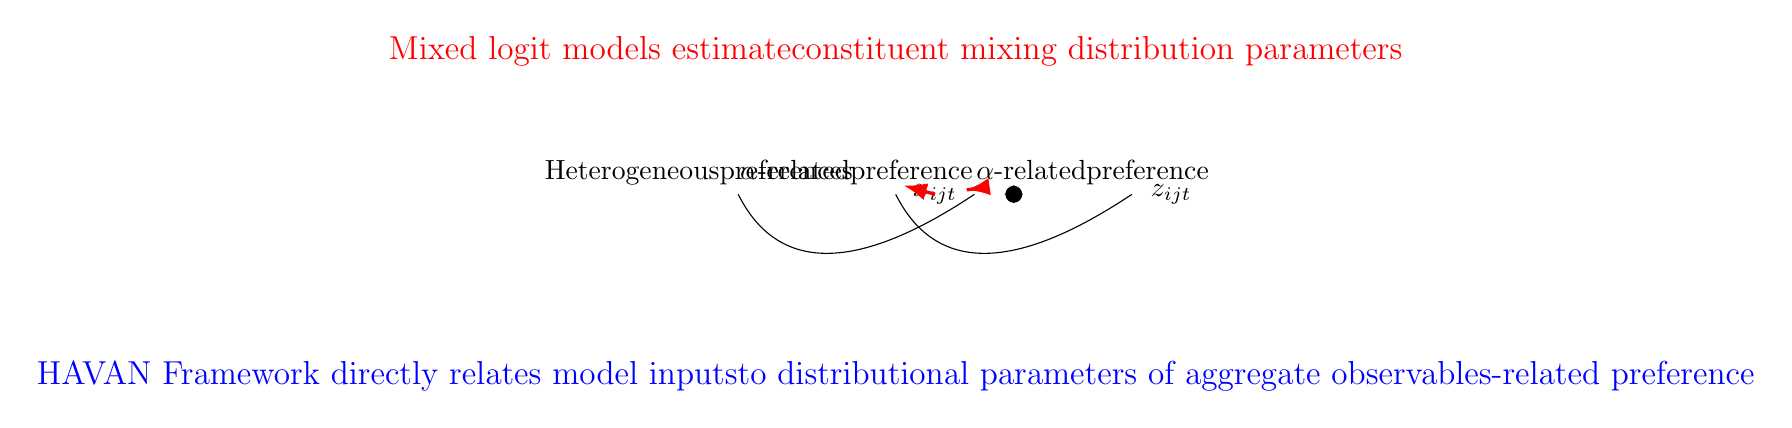
\begin{tikzpicture}[->, >=Latex]
        % Define nodes for the Gaussian distributions
        \node (heterogeneous_preferences) at (-2,0) [above] {Heterogeneous\\preferences};
        \node (alpha_related_preference_1) at (0,0) [above] {$\alpha$-related\\preference};
        \node (x_ijt) at (1,0) {$x_{ijt}$};
        \node (plus) at (2,0) {+};
        \node (alpha_related_preference_2) at (3,0) [above] {$\alpha$-related\\preference};
        \node (z_ijt) at (4,0) {$z_{ijt}$};

        % Draw the Gaussian distributions
        \draw[-] (-1.5,0) .. controls (-1,-1) and (0,-1) .. (1.5,0);
        \draw[-] (0.5,0) .. controls (1,-1) and (2,-1) .. (3.5,0);

        % Draw arrows between the nodes
        \draw[red, very thick, ->] (alpha_related_preference_1) -- node[above] {} (x_ijt);
        \draw[red, very thick, ->] (x_ijt) -- node[above] {} (alpha_related_preference_2);
        
        % Draw the "plus" symbol
        \filldraw (plus) circle (0.1);
        
        % Add the title
        \node[above, red, font=\large] at (0.5,1.5) {Mixed logit models estimate \\ constituent mixing distribution parameters};
        
        % Add the caption
        \node[below, blue, font=\large] at (0.5,-2) {HAVAN Framework directly relates model inputs\\ to distributional parameters of aggregate observables-related preference};
    \end{tikzpicture}
\end{center}

\end{document}